\documentclass[lang=cn,a4paper]{elegantpaper}

\title{基于大数据的老旧小区加装电梯出资分摊方案的数学建模研究}
\author{作者:陶理 \and 指导老师:季鑫}
\institute{上海市实验学校}
\date{\zhtoday}

\usepackage{url,appendix,float,graphicx,diagbox,multicol}

\begin{document}

    \maketitle
    
    \begin{abstract}
        \keywords{老旧小区加装电梯,数学建模,大数据}
    \end{abstract}

    \section{绪论}

    \subsection{背景介绍}

    随着中国城市化进程的不断推进,各地的大规模城市建设正如火如荼地进行。与此同时,各大城市中许多上世纪90年代建造的老旧居民小区已不适应现代的生活需求,其升级改造势在必行。并且,老旧小区在各大城市中的占比很高\cite{research.ke},对于城市的美观有负面影响。所以对于老旧小区的改造势在必行。

    \begin{figure}[H]
        \centering
        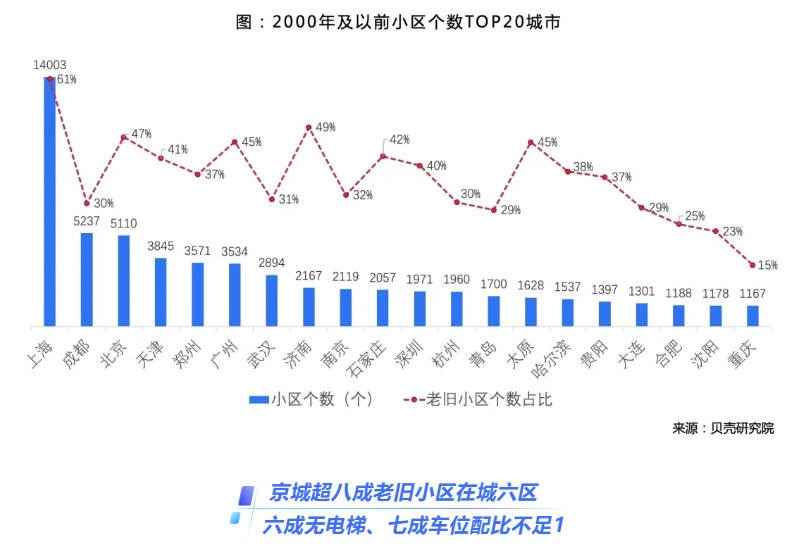
\includegraphics[scale=0.3]{number of old.png}
    \end{figure}
    老旧小区改造中的重要一项是为低层建筑(主要为六层楼房)加装电梯。电梯的安装将极大地方便居民出行和物流服务,特别是在提升深度老龄化群体的生活品质方面具有重要的意义。
    
    在此过程中涉及到一个关键问题是居民的出资分摊方案。除政府补助部分之外,目前一般的方案是按照楼层高度以简单的正比例函数的形式进行分摊,即$C=\dfrac{kL}{N}$\footnote{$C$表示每一户需要分摊的金额;$k$表示分摊系数;\\$L$表示楼层数;$N$表示每层楼的户数}。然而,这一简单方案难以准确反映不同楼层对于加装电梯的实际需求以及后续相关的商业增值。一般来说,较高楼层(5、6楼)原本由于上下楼不方便价值并不显著,但是加装电梯后,高楼层采光等优势愈发明显;低楼层对于电梯的需求本来不大,而且加装电梯后采光的劣势增加。所以各楼户的增值并非与楼层成正比,原本的分摊方案并不科学经济。
    
    \subsection{研究目的}
    提出一个数学模型,形如$f(a_1,a_2,\dots,a_n)=k$,将地段、楼层、居住者年龄/健康情况等各方面影响因素均定量处理作为变量,输出该楼栋加装电梯适宜的分摊比例。

    模型旨在打破常规的正比例函数式分摊比例,用大数据说明事实,更加科学理性地体现各个楼层之间的利益变化量,以更加公平地调和不同楼层之间利益的变化导致的冲突和不愉快。
    \subsection{研究方法}

    \subsubsection{问卷调查法}
    通过问卷\footnote{见附录A、B},调查上海市部分已改造老旧小区的信息和数据:地段信息(如是否靠近地铁/是否为学区房等)、加装电梯前后不同楼层的户主对于自己房产的价值估计、不同楼层对于加装电梯的态度以及支持或者反对的原因。

    问卷调查有着高效率、调查范围广的优点,可以在较短时间内收集到较多的统一特征的数据。但是问卷调查的缺点也十分明显,如果受调查人员范围过广,导致调查结果不能充分反映所调研方面的数据;或者受调查人员填写问卷时十分草率,导致调查数据没有参考意义。因此,本次调查针对上海市已改造老旧小区的户主进行调查,通过联系居委会分发问卷以及在微信朋友圈中转发传播,尽量减少问卷受到受调查者主观情感意愿的影响。

    \subsubsection{建模法}
    通过建立模型的方式对于问卷所收集的数据进行数学分析。建立数学模型的方法能够定量地研究数据之间的关系,从而理性地根据给定的新数据预测新的结果。借助机器学习或者统计图表及其他统计学方法,可以较为简单地发现各种数据之间的联系。但是需要注意防止出现因果关系颠倒,避免研究不相关的两个变量之间的关系。

    \section{问卷分析}
    共有142人参加问卷的调查,其中3份问卷为无效问卷,139份问卷为有效问卷。
    
    通过问卷\footnote{见附录A}的调查,可以从侧面看出现代人对于住房舒适度(本文中具体体现在对于电梯的需求)以及经济方面的考虑程度。

    问卷设计了一个情境:受调查者作为游客,在出游途中选定了一家酒店/民宿,而受到这家酒店/民宿的一些条件的限制,受调查者需要选出最倾向于居住的楼层。由于本文探究的范围是老旧小区,所以规定这家酒店/民宿一共由6层。

    问卷的内容方面共涉及了4个问题,可分为2部分,即控制加装电梯与否,在问卷中即体现为酒店和民宿。“酒店”问题,即初始条件为已经加装了电梯;“民宿”问题,即初始条件为未加装电梯。而在各分类中,通过控制每层楼的房价的变与不变,反映受调查者在出游的舒适体验和经济方面的抉择,进而体现出不同楼层对于加装电梯所能够承受或者愿意付出的经济代价。
    
    由于“酒店”问题的前提条件是已经加装了电梯,可以体现出受调查者对于居住的楼层的主观意愿。在问题3中,可以发现,在控制价格相同,并且加装有电梯的情况下,有66.19\%的受调查者选择了5、6两层,而只有3.6\%的受调查者选择了1、2层。所以可以看出在价格一样的情况下,大部分受调查者选择更高的楼层居住。在问题4中,可以发现,在同时加装有电梯的情况下,如果各层楼的房价(即支出)依次递增且价格波动不小时,有77\%的受调查者选择了1-3层,而其中有60.7\%的受调查者在问题三中选择了5、6两层;而且有37.41\%的受调查者选择了3层。所以可以看出在加装电梯的情况下,价格问题会较大影响居住的选择,但是由于现在人们的条件愈发优越,所以会选择在自己能够承受的范围内的最好的。由“酒店”问题可以看出,如果所居住地有电梯,那么人们倾向于在可承受的经济范围内选择较高的楼层。

    由于“民宿”问题的前提条件是未加装电梯,可以体现出受调查者对于电梯的需求。在问题5中,可以发现79.13\%的受调查者选择了1-3层,其中2层、3层分别占了总体的36.69\%和30.94\%,而4-6层一共只有20.86\%的受调查者选择。在问题6中,可以更明显地发现人们对于低楼层的喜爱。通过这两个问题的数据,与“酒店”问题对比,发现数据分布从5、6层降低至1-3层,可以体现出人们在居住的过程中对于电梯的喜爱和重要需求。

    根据问卷,可以发现在有电梯且价格相同的情况下,人们对于居住楼层的选择普遍偏高,数据大部分分布在5、6两层;在没有电梯且价格相同的情况下,人们一般偏向低楼层(偏中部),数据大部分分布在2、3两层;在有电梯且价格不同的情况下,人们对于居住楼层的选择普遍偏低,数据大部分分布在2、3两层;在没有电梯且价格不同的情况下,就更加体现出对于低楼层的“偏爱”。

    综上所述,楼层高度、电梯和金钱对于人们的居住意愿以及居住体验有比较明显的影响,所以加装电梯对于人们生活水平和生活幸福指数的提高有很大的作用,老旧小区加装电梯的进程势在必行。

    \iffalse
    \begin{figure}[H]
        \centering
        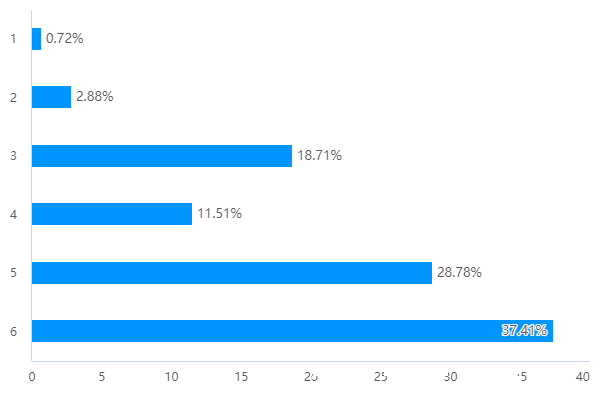
\includegraphics[scale=0.3]{chart_1.png}
    \end{figure}
    \fi

    \section{模型与假设}
    \subsection{符号说明}
    \begin{table}[H]
        \centering
        \begin{tabular}{ccc}
            \toprule
            符号 & 含义 & 单位 \\
            \midrule
            $A_i$ & 未加装电梯时各楼层房价 & 万元\\
            $B_i$ & 加装电梯后各层楼房价 & 万元\\
            $C_i$ & 加装电梯过程中每层楼的花费 & 万元\\
            $A$ & $A=\sum_{i=1}^6A_i$ & 万元\\
            $B$ & $B=\sum_{i=1}^6B_i$ & 万元\\
            $C$ & 电梯总价,即$C=\sum_{i=1}^6C_i$ & 万元\\
            $p_i$ & 各楼层对于加装电梯的正(positive)影响系数 & / \\
            $n_i$ & 各楼层对于加装电梯的负(negative)影响系数 & / \\
            $S_i$ & 各层楼毛利润: $S_i=B_i-A_i$ & 万元\\
            $S$ & 总毛利润: $S=\sum_{i=1}^{6}S_i=\sum_{i=1}^{6}(B_i-A_i)=B-A$ & 万元\\
            \bottomrule
        \end{tabular}
    \end{table}
        
    根据未加装电梯时房价$A_i$分摊:每层楼分摊收益为$\displaystyle N_{1_i}=\frac{A_i}{A}\cdot S-C_i=\frac{A_i}{A}\cdot(B-A)-C_i$。按照相同比例,每层楼应该分摊的电梯的费用为$\displaystyle C_{1_i}=\frac{A_i}{A}\cdot C$。

    根据已加装电梯时房价$B_i$分摊:每层楼分摊收益为$\displaystyle N_{2_i}=\frac{B_i}{B}\cdot S-C_i=\frac{B_i}{B}\cdot(B-A)-C_i$。按照相同比例,每层楼应该分摊的电梯的费用为$\displaystyle C_{1_i}=\frac{B_i}{B}\cdot C$。

    根据加装电梯前后房价差(即收益)$S_i=B_i-A_i$分摊:每层楼分摊收益为$\displaystyle N_{3_i}=\frac{S_i}{S}\cdot S-C_i=S_i-C_i=B_i-A_i-C_i$。按照相同比例,每层楼应该分摊的电梯的费用为$\displaystyle C_{1_i}=\frac{B_i-A_i}{B-A}\cdot C$。

    根据平均收益分摊:$\displaystyle N_{4_i}=\bar{S}-C_i=\frac{S}{6}-C_i=\frac{1}{6}(B-A)-C_i$。
    \section*{致谢}
    在论文完成之际,我想要感谢我的班主任,也是我的指导老师季鑫,季老师。他在问卷调查、统计分析、小论文撰写等方面都给予了很大的帮助,凭借自己的经验也对于我小论文后期的完善有很多的帮助。同时感谢我的同班同学们,他们十分热心地转发了我的问卷,我才得以有比较完善的数据体系。其中特别感谢卢薏安同学,她在我的小论文撰写期间提供了许多思路和建议,对于论文的排版和美化也提出了许多自己的见解和建议。
    
    \clearpage

    \bibliography{reference}
    
    \clearpage
    
    \section*{附录}
    \appendix
 
    \section{关于老旧小区加装电梯的数据和户主态度的调研}
    \begin{enumerate}[1.~~]
        \item 您的性别:
        \item 您的年龄:
        \item 如果您外出游玩,选择了一家酒店。这个酒店一共6层,\textbf{每层楼价格相同},\textbf{且配有电梯},并且假设每层楼都有空余房间。请问您会选择居住在哪一层?
        \item 如果您外出游玩,选择了一家酒店。这个酒店一共6层,\textbf{且配有电梯},并且假设每层楼都有空余房间一楼的价格为100元/晚,六楼的价格为600元/晚,\textbf{随着楼层的增高价格依次递增}。请问您会选择居住在哪一层? 
        \item 如果您外出游玩,选择了一家民宿。这个民宿一共6层,\textbf{每层楼的价格相同},\textbf{但是没有配备电梯},并且假设每层楼都有空余房间。请问您会选择居住在哪一层?
        \item 如果您外出游玩,选择了一家民宿。这个民宿一共6层,\textbf{但是没有配备电梯},并且假设每层楼都有空余房间。一楼的价格为100元/晚,六楼的价格为600元/晚,\textbf{随着楼层的增高价格依次递增}。请问您会选择居住在哪一层?
    \end{enumerate}
    \begin{figure}[H]
        \centering
        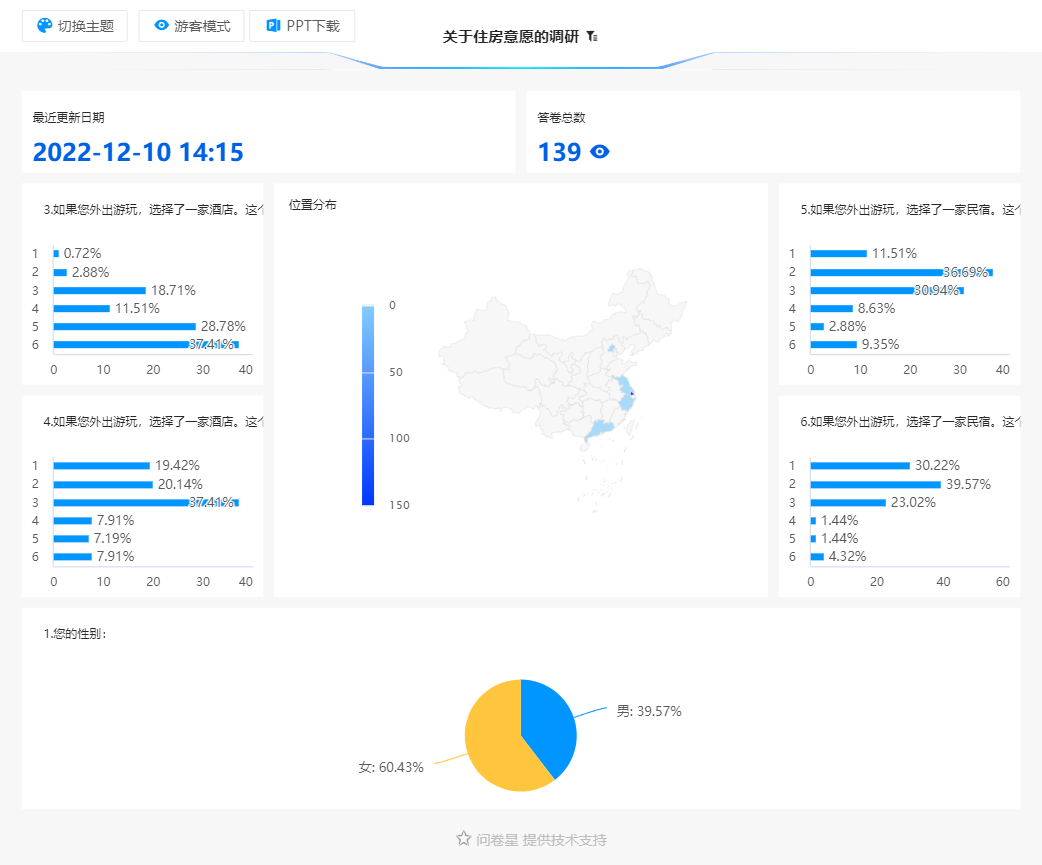
\includegraphics[scale=0.43]{questionnaire.png}
    \end{figure}
\end{document}